\documentclass[a4paper,12pt]{article}
\usepackage{polski}
\usepackage[utf8]{inputenc}
\usepackage{graphicx}
\usepackage{listings}
\usepackage{color}

\definecolor{mygreen}{rgb}{0,0.6,0}
\definecolor{mygray}{rgb}{0.5,0.5,0.5}
\definecolor{mymauve}{rgb}{0.58,0,0.82}

\providecommand{\e}[1]{\ensuremath{\times 10^{#1}}}


\lstset{
    language=c++,
    basicstyle=\footnotesize,
    numberstyle=\footnotesize,
    numbers=left,
    frame=single,
    commentstyle=\color{mygreen},
    tabsize=1,
    title=\lstname,
    escapeinside={\%*}{*)},
    breaklines=true,
    breakatwhitespace=true,
    framextopmargin=2pt,
    framexbottommargin=2pt,
    inputencoding=utf8,
    extendedchars=true,
    literate={ł}{{\/l}}1 {ń}{{\'n}}1,
}
\title{Program typu ping-pong}
\author{Rafał Selewońko}
\begin{document}
\maketitle
 
% pierwsza sekcja
\section{Zadanie}\label{sec:zadanie}
Aplikacja MPI składa się z dwóch procesów: P0 oraz P1. Obydwa procesy 
wymieniają się komunikatami stosując wzorzec wymiany jak w grze w ping-ponga. P0 wysyła 
komunikat do P1 następnie P1 odsyła komunikat do P0. Ta sekwencja wymiany jest powtarzana 
odpowiednią (bardzo dużą) liczbę iteracji, tak aby program wykonywał się przez kilka sekund. Czas 
pracy programu jest obliczany przy pomocy funkcji MPI\_Walltime. Dzieląc ten czas przez liczbę 
iteracji pomnożoną przez dwa (ponieważ komunikat podróżuje w obie strony) otrzymujemy czas 
transmisji komunikatu w jedną stronę. Program powinien wykonywać szereg takich pomiarów dla 
rosnącej długości komunikatów, tak abyś mógł w stanie sporządzić wykres 
czas komunikatu=f(długość). Z kolei dzieląc długość komunikatu przez czas jego transmisji otrzymujemy przepustowość w bajtach/s 
dla danej długości komunikatu. Należy sporządzić również wykres przepustowość=f(długość). 
Program powinien implementować test ping-pong w dwóch wersjach: przy pomocy blokujących 
operacji MPI\_Send/MPI\_Recv oraz przy pomocy nieblokujących MPI\_Isend/MPI\_Recv wraz z 
MPI\_Wait. Wykonaj pomiar na klastrze i sporządź raport z wykonania zadania zawierający wydruk 
programu + obydwa wykresy. Porównaj otrzymane wyniki z wynikiem polecenia ping oraz z 
parametrami sieci Gigabit Ethernet. Porównaj wynik na czas transmisji komunikatu z modelem 
przedstawionym na wykładzie. Czy przy pomocy MPI możliwe jest osiągnięcie maksymalnej 
teoretycznej przepustowości sieci? Jeżeli nie to wymień przyczyny, które Twoim zdaniem to 
uniemożliwiają.
 
\section{Kod programu}\label{sec:kod}

\lstinputlisting{main.cpp}

\section{Wyniki badań}

\begin{table}[t]
\caption{podpis do tabeli}
\label{nazwa odnośnika, która potem użyjemy do cytowania tabeli}
 \begin{tabular}{|r|l|l|l|}
  \hline
  wielkosc & blokujacy & nieblokujacy & ping \\
  \hline
1 & 3.975074\e{-7} & 2.455981\e{-7} &  \\
  \hline
2 & 2.932502\e{-7} & 2.454362\e{-7} &  \\
  \hline
4 & 2.971865\e{-7} & 2.465749\e{-7} &  \\
  \hline
8 & 3.083114\e{-7} & 2.486267\e{-7} &  \\
  \hline
16 & 3.175810\e{-7} & 2.466659\e{-7} & 1.83\e{-7} (24) \\
  \hline
32 & 3.147961\e{-7} & 2.462602\e{-7} & 1.80\e{-7} (40) \\
  \hline
64 & 3.254700\e{-7} & 2.555389\e{-7} & 1.81\e{-7} (72) \\
  \hline
  128 & 3.413152\e{-7} & 2.740780\e{-7} & 4.79\e{-7} (136) \\
  \hline
256 & 3.448095\e{-7} & 2.926863\e{-7} & 4.70\e{-7} (264) \\
  \hline
512 & 4.126596\e{-7} & 3.546302\e{-7} & 5.01\e{-7} (520) \\
  \hline
1024 & 5.276343\e{-7} & 4.776539\e{-7} & 5.16\e{-7} (1032) \\
  \hline
\end{tabular} 
\end{table}

\begin{figure}[ht!]
    \centering
    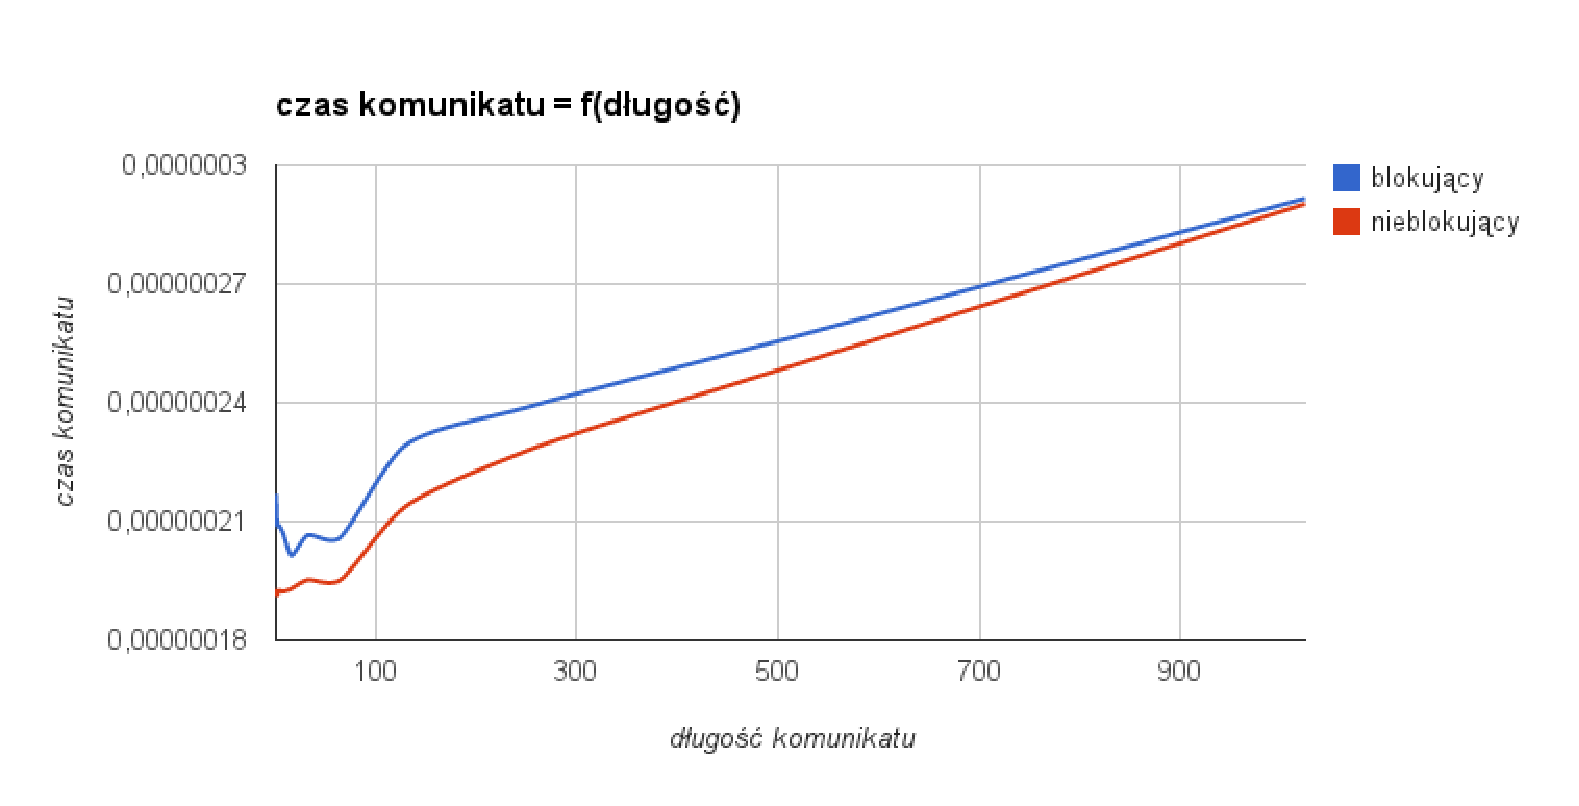
\includegraphics[width=16cm]{wykres_czas.eps}
    \caption{Wykres czasu w zależności od rozmiaru komunikatu.}
    \label{wykres_zas}
\end{figure}

Lorem ipsum dolor sit amet.

\begin{figure}[ht!]
    \centering
    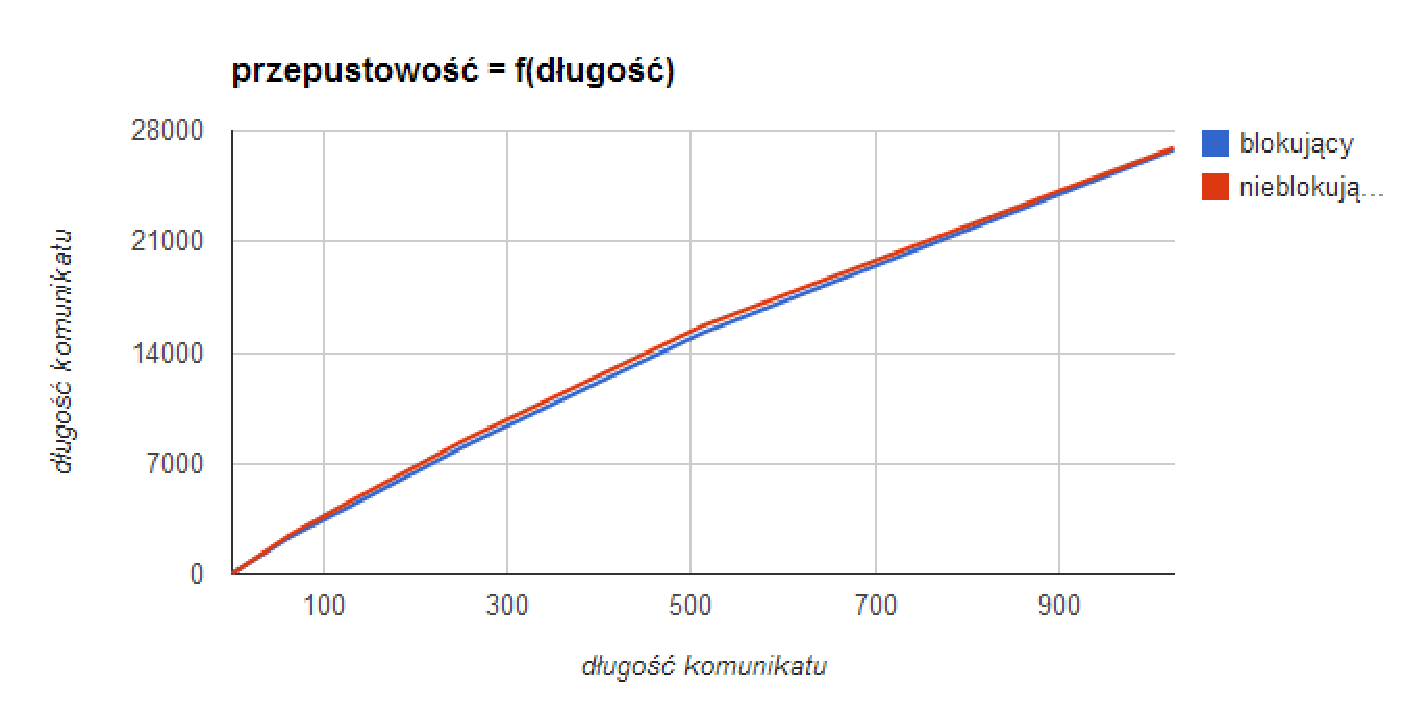
\includegraphics[width=16cm]{wykres_przepustowosc.eps}
    \caption{Wykres przepustowości w zależności od rozmiaru komunikatu.}
    \label{wykres_przepustowosc}
\end{figure}

\subparagraph{podparagraf}
Lorem ipsum dolor sit amet.
\end{document}
